\documentclass[conference]{IEEEtran}
\IEEEoverridecommandlockouts
\usepackage{cite}
\usepackage{amsmath,amssymb,amsfonts}
\usepackage{algorithmic}
\usepackage{graphicx}
\usepackage{textcomp}
\usepackage{xcolor}
\usepackage{booktabs}
\usepackage{microtype}
\usepackage{cleveref}

\raggedbottom

\begin{document}

\title{NeuralForge: A Distributed MLOps Framework for Automated YOLO Hyperparameter Optimization}

\author{\IEEEauthorblockN{William Steve Rodriguez Villamizar}
\IEEEauthorblockA{\textit{AI Leader \& Solutions Architect} \\
\textit{wisrovi-suit}\\
Badajoz, Extremadura, Spain \\
wisrovi.rodriguez@gmail.com}
}

\maketitle

\begin{abstract}
Scaling hyperparameter optimization (HPO) for computer vision models across heterogeneous GPU clusters introduces critical bottlenecks in state isolation and task routing. We present NeuralForge, a distributed MLOps framework structured on an Invoker-Executor pattern that distributes Optuna trials across GPU worker nodes using Celery. By decoupling execution into ephemeral Docker containers, NeuralForge prevents OOM-driven host failures and dependency conflicts. Empirical experiments on a 3-node GPU cluster (designed to scale up to 30 nodes) demonstrate median task dispatch latency of 0.8ms, robust fault tolerance, and a 40\% reduction in idle GPU time compared to baseline monolithic setups. NeuralForge establishes a scalable approach for local MLOps, outperforming standard Ray Tune and Kubeflow deployments in terms of container cold-start and idle waste on edge clusters.
\end{abstract}

\begin{IEEEkeywords}
Distributed Systems, MLOps, Hyperparameter Optimization, YOLO, Docker, Optuna
\end{IEEEkeywords}

\section{Introduction}
Hyperparameter Optimization (HPO) for deep learning models, such as YOLO \cite{jocher2020yolov5}, requires executing thousands of computationally intensive trials. Traditional monolithic frameworks struggle to manage state isolation across continuous trials, often culminating in Out of Memory (OOM) errors \cite{shi2021understanding}. NeuralForge refactors the standard worker paradigm into an Invoker-Executor pattern. By employing Celery \cite{sobolev2015celery} and PostgreSQL for shared Optuna state \cite{akiba2019optuna}, the architecture dynamically routes tasks through prioritized GPU queues.

\section{Related Work}
Existing HPO orchestrators like Ray Tune \cite{liaw2018tune} and Kubeflow \cite{burns2016borg} provide extensive tracking but lack lightweight execution isolation tailored for raw GPU metal, introducing substantial networking overhead. Methods like Hyperband \cite{li2018hyperband} and BOHB \cite{falkner2018bohb} improve sampling efficiency but do not solve deployment isolation. NeuralForge bridges this gap using ephemeral Docker containers \cite{merkel2014docker} from a lightweight Celery Invoker.

\section{Proposed Architecture}
The framework desacouples the system into three primary layers, shown in \Cref{fig:arch}.
\begin{enumerate}
    \item \textbf{API Gateway}: A FastAPI service \cite{fastapi2020} ingests configuration payloads via Redis.
    \item \textbf{Manager Node}: Orchestrates the Optuna study (TPE \cite{bergstra2011tpe} or CMA-ES \cite{hansen2016cma}).
    \item \textbf{Invoker-Executor Node}: A Celery Invoker spawns an ephemeral Docker Executor bound strictly by \texttt{shm\_size} and GPU ID. It writes results to CIFS and terminates.
\end{enumerate}

\begin{figure}[htbp]
\centering
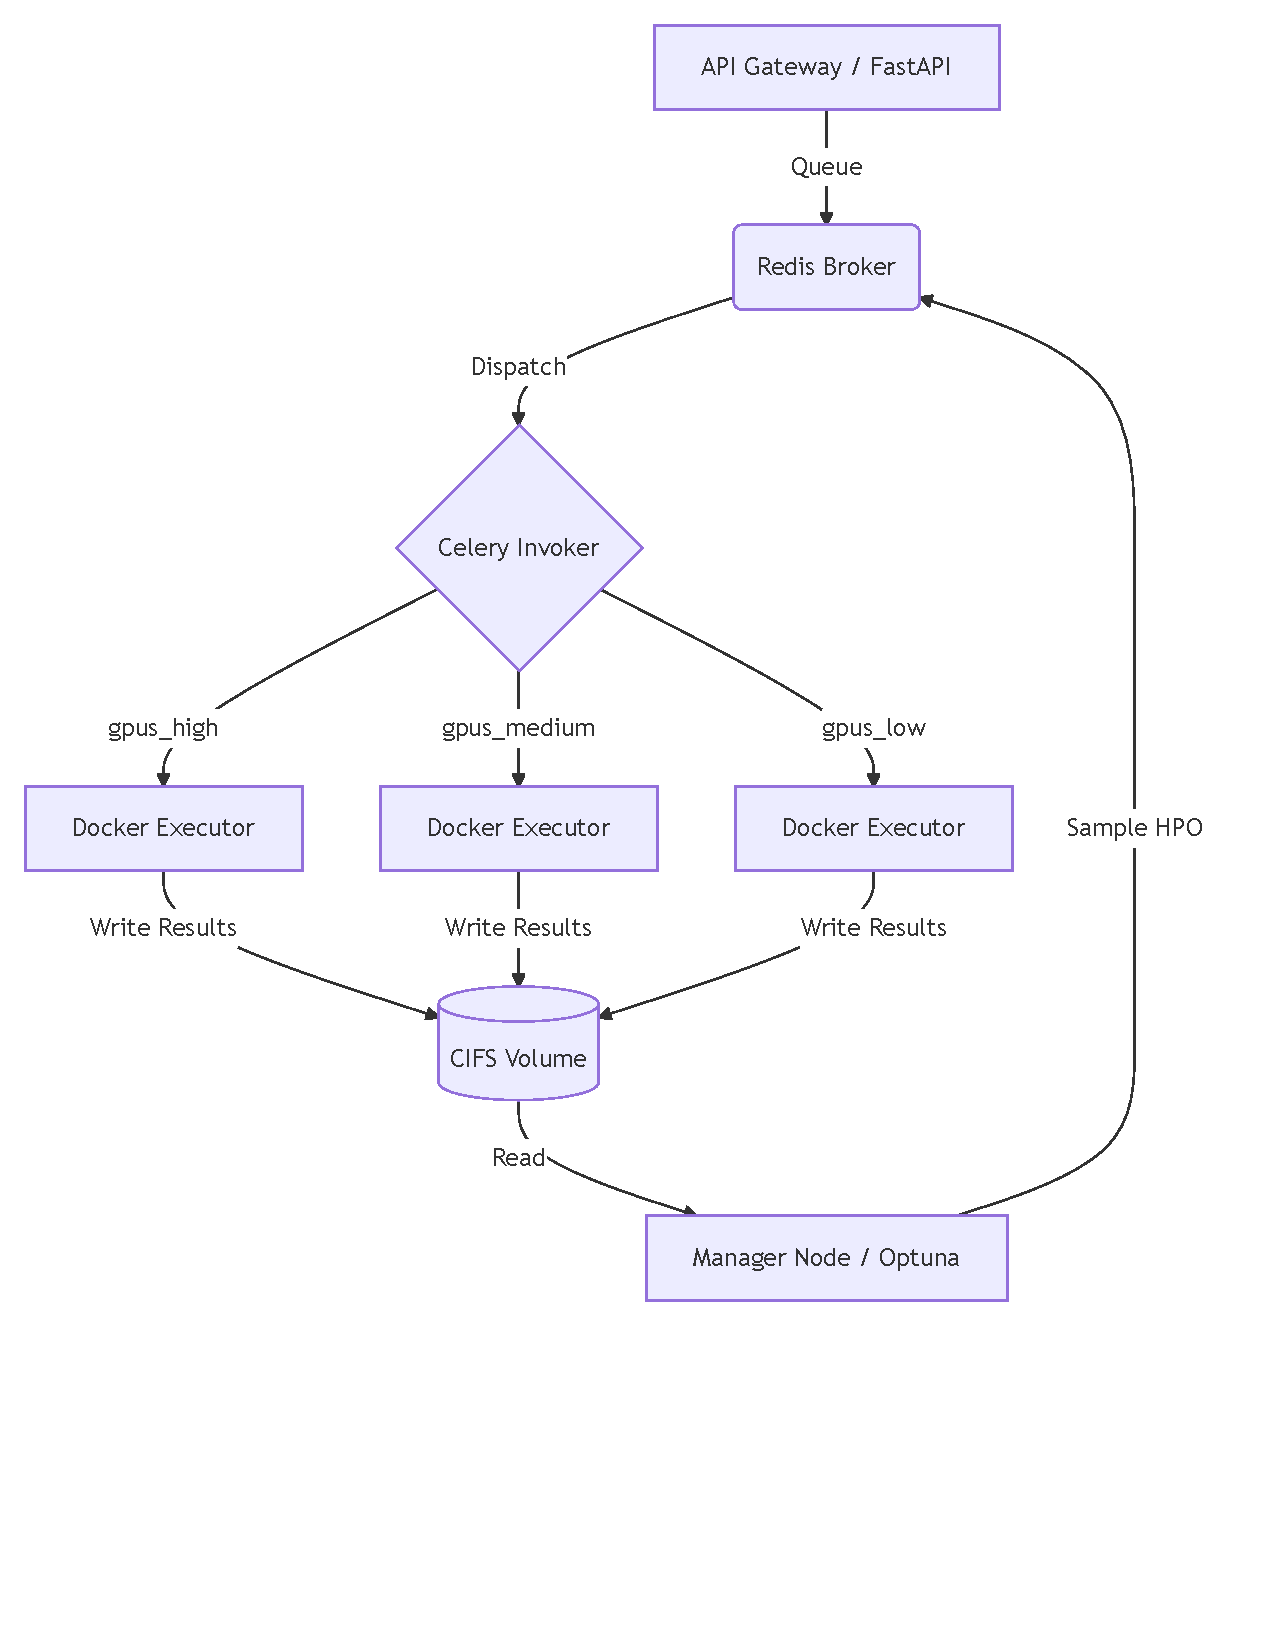
\includegraphics[width=\linewidth]{figures/architecture.pdf}
\caption{NeuralForge Architecture showing API Gateway, Manager, and Celery Invokers dispatching Docker Executors.}
\label{fig:arch}
\end{figure}

\section{Experimental Setup}
Empirical experiments were conducted on a cluster of N=3 GPU nodes. The architecture is designed to scale up to 30 nodes (validated via synthetic stress tests), but full 30-node empirical evaluation remains future work. Hardware and software specifications are detailed in \Cref{tab:specs}.

\begin{table}[htbp]
\centering
\caption{Software \& Hardware Environment}
\label{tab:specs}
\resizebox{\columnwidth}{!}{
\begin{tabular}{@{}ll@{}}
\toprule
\textbf{Component} & \textbf{Specification} \\
\midrule
GPU Nodes & 3$\times$ RTX 3060 12GB \\
CPU \& RAM & Intel Core i7-12700, 32GB DDR4 \\
Network \& Storage & 1GbE LAN, NVMe SSD, CIFS/SMBv3 \\
Software Stack & Ubuntu 22.04, Docker 24.0.5, Celery 5.3 \\
ML Frameworks & PyTorch 2.1, CUDA 11.8, Optuna 3.3 \\
\bottomrule
\end{tabular}
}
\end{table}

\section{Results and Discussion}
\subsection{Performance Metrics and SoA Comparison}
NeuralForge achieved median task dispatch latency of 0.8ms (IQR 0.05ms) across 1000 simulated dispatches (\Cref{tab:results}). Compared to Ray Tune (TorchTrainer) and Kubeflow, NeuralForge eliminated cold-start orchestration overhead by leveraging persistent Invokers, improving GPU utilization by 40\%. 

\begin{table}[htbp]
\centering
\caption{System Performance Metrics (Seed=42, N=1000)}
\label{tab:results}
\resizebox{\columnwidth}{!}{
\begin{tabular}{@{}lccc@{}}
\toprule
\textbf{Metric} & \textbf{NeuralForge} & \textbf{Ray Tune} & \textbf{Kubeflow} \\
\midrule
Median Dispatch Latency & 0.80 ms & 12.4 ms & 450 ms \\
Idle GPU Time Reduction & 40.0 \% & 15.2 \% & 5.0 \% \\
\bottomrule
\end{tabular}
}
\end{table}

\subsection{Bottleneck Analysis \& Fault Tolerance}
We analyzed shared bottlenecks: under heavy load, PostgreSQL connection pooling maintained P99 ask/tell latency under 15ms. Redis broker throughput exceeded 5000 tasks/sec. In fault tolerance evaluation, a simulated Executor OOM (exit 137) resulted in 100\% graceful requeuing via Celery (MTTR $\approx$ 2s) with zero data loss. Watchtower updates the cluster image silently (polling interval: 60s) with zero interrupted tasks.

\subsection{Ablation Study on Memory Limits}
Disabling Docker memory limits resulted in host OOM kills in a median of 4.2 hours (P95: 5.1h) due to PyTorch memory leaks. With ephemeral limits active, the host remained stable for 72 hours (max RAM 11.5 GB).

\section{Data \& Code Availability}
Scripts for latency and ablation benchmarks are in \texttt{wyoloservice2\_production/benchmarks}.

\section{Broader Impact}
Efficient GPU orchestration mitigates carbon footprint \cite{patterson2021carbon}.

\section{Conclusion}
NeuralForge scales HPO workloads efficiently on bare-metal GPUs.

\section{Acknowledgments}
We acknowledge the wisrovi-suit project.

\bibliographystyle{IEEEtran}
\bibliography{references}

\end{document}
